
%\documentclass[a4paper,11pt]{article}
\documentclass{article}

\usepackage[hangul]{kotex}
\usepackage{enumitem}
\usepackage{mathtools}
\usepackage{stmaryrd}
\usepackage{float}
\usepackage{multirow}
\usepackage{array}
\usepackage[margin=1in, bottom=1in]{geometry}

%\usepackage[bitstream-charter]{mathdesign}
%\usepackage[T1]{fontenc}

\setlength{\hoffset}{-25pt}
\addtolength{\textwidth}{50pt}
\setlength{\voffset}{-60pt}
\addtolength{\textheight}{130pt}

\newcommand{\w}[1]{\ensuremath{\textit{#1}}}
\newcommand{\x}{\times}
\newcommand{\rem}{\mtt{\%}}
\newcommand{\rar}{\rightarrow}
\newcommand{\Rar}{\Rightarrow}
\newcommand{\U}{\cup}
\newcommand{\join}{\sqcup}
\newcommand{\ttt}[1]{\texttt{#1}}
\newcommand{\mtt}[1]{\mathtt{#1}}
\newcommand{\bigspace}{\,\,\,\,\,\,\,\,}

\newcommand{\op}[2]{\mtt{#1(}#2\mtt{)}}
\newcommand{\module}[3]{\mtt{#1(}#2\mtt{)(}#3\mtt{)}}
\newcommand{\conc}{\mtt{@}}
\newcommand{\ind}[1]{\mtt{[}#1\mtt{]}}
\newcommand{\indr}[2]{\mtt{[}#1\mtt{:}#2\mtt{]}}
\newcommand{\ifs}[3]{\mtt{if}\,\,#1\,\,\mtt{then}\,\,#2\,\,\mtt{else}\,\,#3}

\newenvironment{prepost}[4]{
  \begin{tabular}{|>{\centering}m{0.4\textwidth}|p{0.6\textwidth}|}
    \hline
    \multicolumn{2}{|l|}{\texttt{#1}} \\ \hline
      \multirow{4}{*}{#2}
     & Require \\ \cline{2-2}
     & #3 \\ \cline{2-2}
     & Guarantees \\ \cline{2-2}
     & #4 \\ \hline
  \end{tabular}
}

\newenvironment{prepostc}[5]{
  \begin{tabular}{|>{\centering}m{0.4\textwidth}|p{0.6\textwidth}|}
    \hline
    \multicolumn{2}{|l|}{\texttt{#1}} \\ \hline
      \multirow{6}{*}{#2}
     & Require \\ \cline{2-2}
     & #3 \\ \cline{2-2}
     & Guarantees \\ \cline{2-2}
     & #4 \\ \cline{2-2}
     & Comment\\ \cline{2-2}
     & #5 \\ \hline
  \end{tabular}
}

\newenvironment{onlyc}[3]{
  \begin{tabular}{|>{\centering}m{0.4\textwidth}|p{0.6\textwidth}|}
    \hline
    \multicolumn{2}{|l|}{\texttt{#1}} \\ \hline
      \multirow{2}{*}{#2}
     & Comment\\ \cline{2-2}
     & #3 \\ \hline
  \end{tabular}
}

\newenvironment{itemizec}{
  \begin{itemize}
}{
  \end{itemize}
  \quad
  \vspace{-1em}
}


\begin{document}

\setlist{nolistsep}
\nointerlineskip
\par\noindent
\setlength{\parindent}{0pt}


\subsection*{\texttt{torch.Tensor.size}}%{{{
\prepost{a.size()}{
  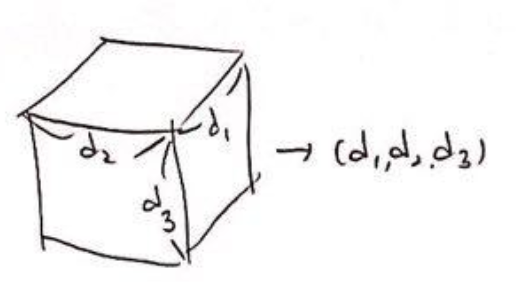
\includegraphics[height=8em]{resources/size1.png}
}{
  \begin{itemizec}
    \item $|\mtt{a}| = (d_1, d_2, \dots, d_k)$
  \end{itemizec}
}{
  \begin{itemizec}
    \item $(d_1, d_2, \dots, d_k)$를 튜플로 반환
  \end{itemizec}
}
\begin{align*}
  \frac
  {
    \begin{array}{l}
      \sigma \vdash E \Rar e, c
    \end{array}
  }
  {
    \sigma \vdash E.\op{size}{} \Rar shapeToTuple(e), c
  }
\end{align*}

\prepost{a.size(n)}{
  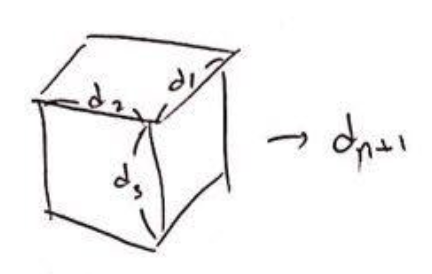
\includegraphics[height=8em]{resources/size2.png}
}{
  \begin{itemizec}
    \item $|\mtt{a}| = (d_1, d_2, \dots, d_k)$
    \item $0 \leq n < k$
  \end{itemizec}
}{
  \begin{itemizec}
    \item $d_{n+1}$을 숫자(int)로 반환
  \end{itemizec}
}
\begin{align*}
  \frac
  {
    \begin{array}{l}
      \sigma \vdash E \Rar e, c \\
      k = \op{rank}{e} \\
      c' = \{ (k \geq 1) \land (0 \leq n < k) \}
    \end{array}
  }
  {
    \sigma \vdash E.\op{size}{n} \Rar e\ind{n+1}, c \cup c'
  }
\end{align*}%}}}

\subsection*{\texttt{torch.tensor}}%{{{
\onlyc{torch.tensor(x)}{
}{\texttt{numpy}나 파이썬 리스트로 선언된 객체를
\texttt{torch}에서 호환가능한 형태로 바꾸는 함수.}
\begin{align*}
  \frac
  {
    \sigma \vdash {E} \Rar e, c
  }
  {
    \sigma \vdash \op{tensor}{E} \Rar e, c
  }
\end{align*}%}}}

\subsection*{\texttt{torch.Tensor.shape}}%{{{
\prepost{a.shape}{
  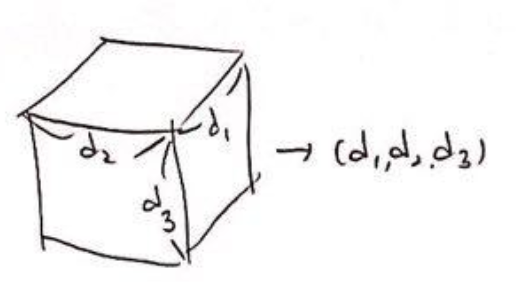
\includegraphics[height=8em]{resources/size1.png}
}{
  \begin{itemizec}
    \item $|\mtt{a}| = (d_1, d_2, \dots, d_k)$
  \end{itemizec}
}{
  \begin{itemizec}
    \item $(d_1, d_2, \dots, d_k)$를 튜플로 반환
  \end{itemizec}
}
\begin{align*}
  \frac
  {
    \begin{array}{l}
      \sigma \vdash E \Rar e, c
    \end{array}
  }
  {
    \sigma \vdash E.\mtt{shape} \Rar shapeToTuple(e), c
  }
\end{align*}%}}}

\subsection*{\texttt{torch.range}}%{{{
\prepostc{torch.range(s, e, d)}{
  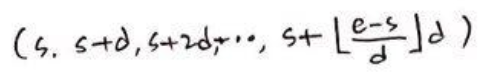
\includegraphics[width=\linewidth]{resources/range.png}
}{
  \begin{itemizec}
    \item $d \neq 0$
    \item $(e-s)/d > 0$
  \end{itemizec}
}{
  \begin{itemizec}
    \item $|y| = (1 + (e-s)/d)$
  \end{itemizec}
}{
  \begin{itemizec}
      \item $(s, s+d, s+2d, \dots)$를 반환
      \item 기본값은 $s = 0$, $d = 1$
    \end{itemizec}
}
\begin{align*}
  \frac
  {
    \begin{array}{l}
      c = \{(d \neq 0) \land ((e-s)/d > 0)\}
    \end{array}
  }
  {
    \sigma \vdash \op{range}{s, e, d} \Rar (1+\lfloor (e-s)/d \rfloor), c
  }
  \tag*{Default: $s = 0, d = 1$}
\end{align*}%}}}

\subsection*{\texttt{torch.Tensor.item}}%{{{
\prepostc{a.item()}{
  
\includegraphics[width=\linewidth]{resources/item.png}
}{
  \begin{itemizec}
    \item $|a| = ()$ or $|a| = (1, 1, 1, \dots, 1)$
  \end{itemizec}
}{
  \begin{itemizec}
    \item $|y| = e_n$
  \end{itemizec}
}{
  \begin{itemizec}
    \item Singular element tensor의 원소(스칼라 타입으로 반환)
  \end{itemizec}
}
\begin{align*}
  \frac
  {
    \begin{array}{l}
      \sigma \vdash E \Rar e, c \\
      k = \op{rank}{e} \\
      c' = \{ (\forall i = 1, 2, \dots, k,\: e[i] = 1) \}
    \end{array}
  }
  {
    \sigma \vdash E.\op{item}{} \Rar e_n, c \cup c'
  }
\end{align*}%}}}

\subsection*{\texttt{torch.split}}%{{{
\prepostc{torch.split(x, n, p=0)}{
  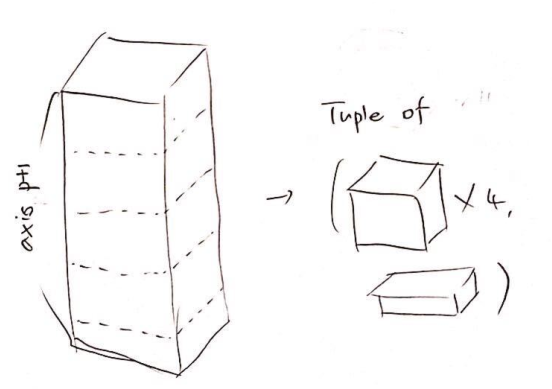
\includegraphics[height=14em]{resources/split1.png}
}{
  \begin{itemizec}
    \item $|x| = (d_1, d_2, \dots, d_k)$
    \item $k \geq 1$
    \item $0 \leq p < k$
  \end{itemizec}
}{
  \begin{itemizec}
    \item 아래 proof tree와 같이 $p+1$번째 axis가 최대 $n$개의 원소를 가지도록
    $\lceil d_{p+1} / n \rceil$개 튜플 형태로 반환
  \end{itemizec}
}{
  \begin{itemizec}
    \item Concat의 반대 역할 함수
    \item Divisible 여부 assert하지 않음
    \item 학습 및 테스트 데이터를 배치단위로 쪼개는 용도로 쓰일 것으로 추측
  \end{itemizec}
}
\begin{align*}
  \frac
  {
    \begin{array}{l}
      \sigma \vdash E \Rar e, c \\
      k = \op{rank}{e} \\
      e_1 = e\indr{1}{p} \conc (n) \conc e\indr{p+2}{k} \\
      e_2 = e\indr{1}{p} \conc (n) \conc e\indr{p+2}{k} \\
      \bigspace \cdots \\
      e_{l-1} = e\indr{1}{p} \conc (n) \conc e\indr{p+2}{k} \\
      e_l = e\indr{1}{p} \conc (n') \conc e\indr{p+2}{k} \bigspace
        \text{where $e \ind{p+1} = n(l-1) + n'$, $0 < n' \leq n$} \\
      c' = \{ (k \geq 1) \land (0 \leq p < k) \}
    \end{array}
  }
  {
    \sigma \vdash \op{split}{E, n, p=0} \Rar (e_1, e_2, \dots, e_l), c \cup c'
  }
  \tag*{$l$-원소 tuple 형태로 반환}
\end{align*}

\prepost{torch.split(x, [n1, n2, ..., nl], p=0)}{
  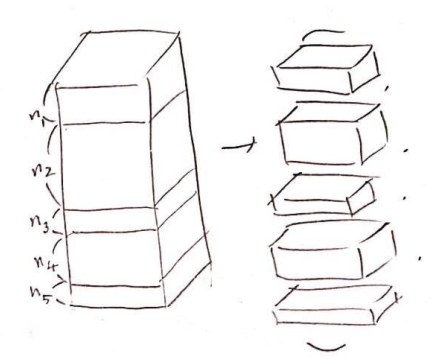
\includegraphics[height=14em]{resources/split2.png}
}{
  \begin{itemizec}
    \item $|x| = (d_1, d_2, \dots, d_k)$
    \item $k \geq 1$
    \item $0 \leq p < k$
    \item $d_{p+1} = n_1 + n_2 + \cdots + n_l$
  \end{itemizec}
}{
  \begin{itemizec}
    \item 아래 proof tree와 같이 $p+1$번째 axis의 크기가 $n_1, n_2, \dots, n_l$인
    $l$개의 텐서 튜플을 반환
    \item $n_i$의 합과 $d_{p+1}$이 같은지 assert
  \end{itemizec}
}
\begin{align*}
  \frac
  {
    \begin{array}{l}
      \sigma \vdash E \Rar e, c \\
      k = \op{rank}{e} \\
      e_1 = e\indr{1}{p} \conc (n_1) \conc e\indr{p+2}{k} \\
      e_2 = e\indr{1}{p} \conc (n_2) \conc e\indr{p+2}{k} \\
      \bigspace \cdots \\
      e_l = e\indr{1}{p} \conc (n_l) \conc e\indr{p+2}{k} \\
      c' = \{ (k \geq 1) \land (0 \leq x < k) \land
        (e \ind{p+1} = n_1 + n_2 + \cdots + n_l) \}
    \end{array}
  }
  {
    \sigma \vdash \op{split}{E, \ind{n_1, n_2, \dots, n_l}, p=0}
      \Rar (e_1, e_2, \dots, e_l), c \cup c'
  }
  \tag*{$l$-원소 tuple 형태로 반환}
\end{align*}%}}}

\subsection*{\texttt{torch.zeros}, \texttt{torch.rand}, \texttt{torch.randn}}%{{{
\prepostc{torch.zeros(t1, t2, ..., tl) or .rand, .randn}{
}{
}{
  \begin{itemizec}
    \item $|y| = (t_1, t_2, \dots, t_l)$
  \end{itemizec}
}{
  \begin{itemizec}
    \item 입력받은 형태대로 $0$, uniformly random, gaussian random 텐서를 반환
  \end{itemizec}
}
\begin{align*}
  \forall \mtt{ft} \in \{\mtt{zeros}, \mtt{rand}, \mtt{randn}\},
  \bigspace
  \frac
  {
  }
  {
    \sigma \vdash \op{ft}{t_1, t_2, \dots, t_l} \Rar (t_1, t_2, \dots, t_l),
      \emptyset
  }
\end{align*}%}}}

\subsection*{\texttt{torch.mode}}%{{{
\prepostc{torch.mode(x, n=0, keep\_dim=False)}{
  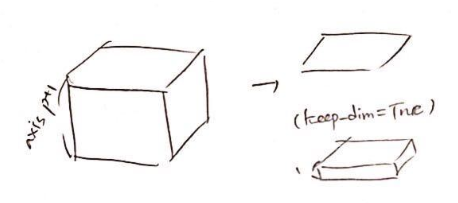
\includegraphics[height=8em]{resources/reduce.png}
}{
  \begin{itemizec}
    \item $|x| = (d_1, d_2, \dots, d_k)$
    \item $k \geq 1$
    \item $0 \leq n < k$
  \end{itemizec}
}{
  \begin{itemizec}
    \item $|y| = |z| = (d_1, d_2, \dots, d_n, d_{n+2}, \dots, d_k)$인 $(y, z)$
    튜플 반환
    \item 세 번째 인자 $keep\_dim$이 $True$이면 $|y| = |z| = (d_1, d_2, \dots,
    d_n, 1, d_{n+2}, \dots, d_k)$
  \end{itemizec}
}{
  \begin{itemizec}
    \item 입력받은 축을 기준으로한 통계적 최빈값 계산 함수
  \end{itemizec}
}
\begin{align*}
  \frac
  {
    \begin{array}{l}
      \sigma \vdash E \Rar e, c \\
      k = \op{rank}{e} \\
      e' = e \indr{1}{n} \conc e \indr{n+2}{k} \\
      c' = \{ (k \geq 1) \land (0 \leq n < k) \}
    \end{array}
  }
  {
    \sigma \vdash \op{mode}{E, n=0} \Rar (e', e'), c \cup c'
  }
  \tag*{tuple 형태로 반환}
\end{align*}

\begin{align*}
  \frac
  {
    \begin{array}{l}
      \sigma \vdash E \Rar e, c \\
      k = \op{rank}{e} \\
      e' = e \indr{1}{n} \conc (1) \conc e \indr{n+2}{k} \\
      c' = \{ (k \geq 1) \land (0 \leq n < k) \}
    \end{array}
  }
  {
    \sigma \vdash \op{mode}{E, n=0, True} \Rar (e', e'), c \cup c'
  }
  \tag*{tuple 형태로 반환}
\end{align*}

\begin{align*}
  \frac
  {
    \sigma \vdash \op{mode}{E, n} \Rar (e, e), c
  }
  {
    \sigma \vdash \op{mode}{E, n=0, False} \Rar (e, e), c
  }
  \tag*{tuple 형태로 반환}
\end{align*}%}}}

\subsection*{\texttt{torch.randint}}%{{{
\prepost{torch.randint(low=0, high, shape)}{
}{
  \begin{itemizec}
    \item $low < high$
    \item $shape$이 well-defined인 텐서 shape. (스칼라 타입은 X)
  \end{itemizec}
}{
  \begin{itemizec}
    \item $|y| = shape$
  \end{itemizec}
}
\begin{align*}
  \frac
  {
    low < high
  }
  {
    \sigma \vdash \op{randint}{low=0, high, s} \Rar tupleToShape(s), \emptyset
  }
\end{align*}%}}}

\subsection*{\texttt{torch.max}, \texttt{torch.min}}%{{{
\prepostc{torch.max(x) or .min}{
  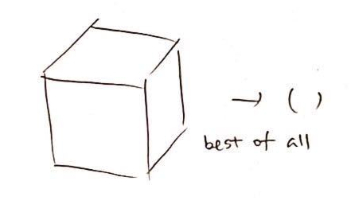
\includegraphics[height=8em]{resources/bestofall.png}
}{
}{
  \begin{itemizec}
    \item $|y| = ()$
  \end{itemizec}
}{
  \begin{itemizec}
    \item 주어진 텐서에서 최대/최소 값을 $()$-shape 텐서로 반환(스칼라 X)
  \end{itemizec}
}
\begin{align*}
  \forall \mtt{ft} \in \{\mtt{min}, \mtt{max}\},
  \bigspace
  \frac
  {
    \begin{array}{l}
      \sigma \vdash E \Rar \_, c
    \end{array}
  }
  {
    \sigma \vdash \op{ft}{E} \Rar (), c
  }
\end{align*}

\prepostc{torch.max(x, n, keep\_dim=False) or .min}{
  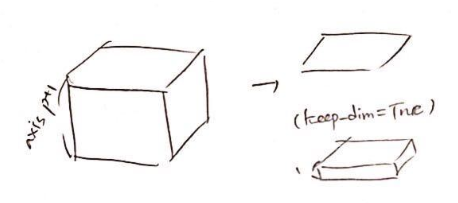
\includegraphics[height=8em]{resources/reduce.png}
}{
  \begin{itemizec}
    \item $|x| = (d_1, d_2, \dots, d_k)$
    \item $k \geq 1$, $0 \leq n < k$
  \end{itemizec}
}{
  \begin{itemizec}
    \item $|y| = |z| = (d_1, d_2, \dots, d_n, d_{n+2}, \dots, d_k)$인 $(y, z)$
    튜플 반환
    \item 세 번째 인자 $keep\_dim$이 $True$이면 $|y| = |z| = (d_1, d_2, \dots,
    d_n, 1, d_{n+2}, \dots, d_k)$
  \end{itemizec}
}{
  \begin{itemizec}
    \item 주어진 텐서에서 축 상의 최대/최소값과, 그에 해당하는 인덱스 번호를
    쌍으로 엮어 튜플로 반환
  \end{itemizec}
}
\begin{align*}
  \forall \mtt{ft} \in \{\mtt{min}, \mtt{max}\},
  \bigspace
  \frac
  {
    \begin{array}{l}
      \sigma \vdash E \Rar e, c \\
      k = \op{rank}{e} \\
      e' = e \indr{1}{n} \conc e \indr{n+2}{k} \\
      c' = \{ (k \geq 1) \land (0 \leq n < k) \}
    \end{array}
  }
  {
    \sigma \vdash \op{ft}{E, n} \Rar (e', e'), c \cup c'
  }
  \tag*{tuple 형태로 반환}
\end{align*}

\begin{align*}
  \forall \mtt{ft} \in \{\mtt{min}, \mtt{max}\},
  \bigspace
  \frac
  {
    \begin{array}{l}
      \sigma \vdash E \Rar e, c \\
      k = \op{rank}{e} \\
      e' = e \indr{1}{n} \conc (1) \conc e \indr{n+2}{k} \\
      c' = \{ (k \geq 1) \land (0 \leq n < k) \}
    \end{array}
  }
  {
    \sigma \vdash \op{ft}{E, n, True} \Rar (e', e'), c \cup c'
  }
  \tag*{tuple 형태로 반환}
\end{align*}

\begin{align*}
  \forall \mtt{ft} \in \{\mtt{min}, \mtt{max}\},
  \bigspace
  \frac
  {
    \sigma \vdash \op{ft}{E, n} \Rar (e, e), c
  }
  {
    \sigma \vdash \op{ft}{E, n, False} \Rar (e, e), c
  }
  \tag*{tuple 형태로 반환}
\end{align*}

\prepostc{torch.max(x, y) or .min}{
  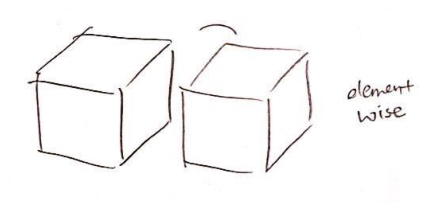
\includegraphics[height=8em]{resources/elementwise.png}
}{
  \begin{itemizec}
    \item $broadcastable(|x|, |y|)$
  \end{itemizec}
}{
  \begin{itemizec}
    \item $broadcast(|x|, |y|)$
  \end{itemizec}
}{
  \begin{itemizec}
    \item 두 텐서의 elementwise 최대/최소
  \end{itemizec}
}
\begin{align*}
  \forall \mtt{ft} \in \{\mtt{min}, \mtt{max}\},
  \bigspace
  \frac
  {
    \begin{array}{l}
      \sigma \vdash E_1 \Rar e_1, c_1 \\
      \sigma \vdash E_2 \Rar e_2, c_2
    \end{array}
  }
  {
    \sigma \vdash \op{ft}{E_1, E_2} \Rar broadcast(e_1, e_2),
      c_1 \cup c_2 \cup broadcastable(e_1, e_2)
  }
\end{align*}%}}}

\subsection*{\texttt{torch.sum}, \texttt{torch.mean}}%{{{
\prepostc{torch.sum(x) or .mean}{
  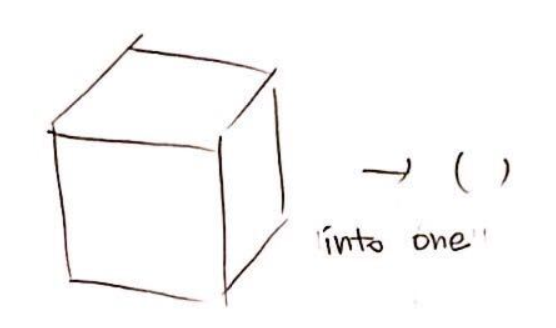
\includegraphics[height=8em]{resources/intoone.png}
}{
  \begin{itemizec}
    \item $\mtt{.mean}$에 대해서는 텐서 타입이 floating이어야 함
  \end{itemizec}
}{
  \begin{itemizec}
    \item $|y| = ()$
  \end{itemizec}
}{
  \begin{itemizec}
    \item 주어진 텐서의 합계/평균값을 $()$-shape 텐서로 반환(스칼라 X)
  \end{itemizec}
}
\begin{align*}
  \forall \mtt{ft} \in \{\mtt{sum}, \mtt{mean}\},
  \bigspace
  \frac
  {
    \begin{array}{l}
      \sigma \vdash E \Rar \_, c
    \end{array}
  }
  {
    \sigma \vdash \op{ft}{E} \Rar (), c
  }
\end{align*}

\prepostc{torch.sum(x, n, keep\_dim=False) or .mean}{
  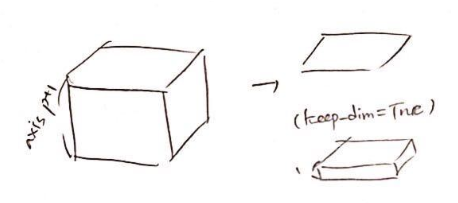
\includegraphics[height=8em]{resources/reduce.png}
}{
  \begin{itemizec}
    \item $|x| = (d_1, d_2, \dots, d_k)$
    \item $k \geq 1$, $0 \leq n < k$
    \item $\mtt{.mean}$에 대해서는 텐서 타입이 floating이어야 함
  \end{itemizec}
}{
  \begin{itemizec}
    \item $|y| = (d_1, d_2, \dots, d_n, d_{n+2}, \dots, d_k)$
    \item 세 번째 인자 $keep\_dim$이 $True$이면 $|y| = (d_1, d_2, \dots,
    d_n, 1, d_{n+2}, \dots, d_k)$
  \end{itemizec}
}{
  \begin{itemizec}
    \item 주어진 텐서에서 축 상의 합/평균을 반환
  \end{itemizec}
}
\begin{align*}
  \forall \mtt{ft} \in \{\mtt{sum}, \mtt{mean}\},
  \bigspace
  \frac
  {
    \begin{array}{l}
      \sigma \vdash E \Rar e, c \\
      k = \op{rank}{e} \\
      e' = e \indr{1}{n} \conc e \indr{n+2}{k} \\
      c' = \{ (k \geq 1) \land (0 \leq n < k) \}
    \end{array}
  }
  {
    \sigma \vdash \op{ft}{E, n} \Rar e', c \cup c'
  }
\end{align*}

\begin{align*}
  \forall \mtt{ft} \in \{\mtt{sum}, \mtt{mean}\},
  \bigspace
  \frac
  {
    \begin{array}{l}
      \sigma \vdash E \Rar e, c \\
      k = \op{rank}{e} \\
      e' = e \indr{1}{n} \conc (1) \conc e \indr{n+2}{k} \\
      c' = \{ (k \geq 1) \land (0 \leq n < k) \}
    \end{array}
  }
  {
    \sigma \vdash \op{ft}{E, n, True} \Rar e', c \cup c'
  }
\end{align*}

\prepostc{torch.sum(x, [n1, n2, ..., nl], keep\_dim=False) or .mean}{
  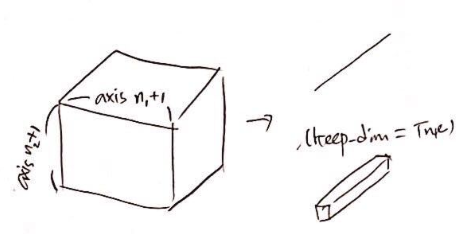
\includegraphics[height=10em]{resources/reduce_multi.png}
}{
  \begin{itemizec}
    \item $|x| = (d_1, d_2, \dots, d_k)$
    \item $k \geq 1$, $0 \leq n < k$
    \item $\mtt{.mean}$에 대해서는 텐서 타입이 floating이어야 함
  \end{itemizec}
}{
  \begin{itemizec}
    \item $|y| = (d_{i_1}, d_{i_2}, \dots, d_{i_{k-l}})$
    \begin{itemize}
      \item $1, 2, \dots, k$에서 $n_1+1, n_2+1, \dots, n_l+1$번째 항이 지워진 shape
    \end{itemize}
    \item 세 번째 인자 $keep\_dim$이 $True$이면 $n_1+1, n_2+1, \dots, n_l+1$번째
    항은 삭제되지 않고 $1$로 남음
  \end{itemizec}
}{
  \begin{itemizec}
    \item 주어진 텐서에서 여러 축을 통합한 합/평균을 반환
  \end{itemizec}
}
\begin{align*}
  \forall \mtt{ft} \in \{\mtt{sum}, \mtt{mean}\},
  \bigspace
  \frac
  {
    \begin{array}{l}
      \sigma \vdash E \Rar e, c \\
      k = \op{rank}{e} \\
      e_1 = \ifs{0 \in \{n_1, n_2, \dots, n_r\}}{()}{(e[1])} \\
      e_2 = \ifs{1 \in \{n_1, n_2, \dots, n_r\}}{()}{(e[2])} \\
      \bigspace \cdots \\
      e_k = \ifs{k-1 \in \{n_1, n_2, \dots, n_r\}}{()}{(e[k])} \\
      e' = e_1 \conc e_2 \conc \cdots \conc e_k \\
      c' = \{ (k \geq 1) \land (\forall i=1, 2, \dots, r,\: 0 \leq n_i < k) \}
    \end{array}
  }
  {
    \sigma \vdash \op{ft}{E, (n_1, n_2, \dots, n_r)} \Rar e', c \cup c'
  }
\end{align*}

\begin{align*}
  \forall \mtt{ft} \in \{\mtt{sum}, \mtt{mean}\},
  \bigspace
  \frac
  {
    \begin{array}{l}
      \sigma \vdash E \Rar e, c \\
      k = \op{rank}{e} \\
      e_1 = \ifs{0 \in \{n_1, n_2, \dots, n_r\}}{(1)}{(e[1])} \\
      e_2 = \ifs{1 \in \{n_1, n_2, \dots, n_r\}}{(1)}{(e[2])} \\
      \bigspace \cdots \\
      e_k = \ifs{k-1 \in \{n_1, n_2, \dots, n_r\}}{(1)}{(e[k])} \\
      e' = e_1 \conc e_2 \conc \cdots \conc e_k \\
      c' = \{ (k \geq 1) \land (\forall i=1, 2, \dots, r,\: 0 \leq n_i < k) \}
    \end{array}
  }
  {
    \sigma \vdash \op{ft}{E, (n_1, n_2, \dots, n_r), True} \Rar e', c \cup c'
  }
\end{align*}

\prepostc{torch.sum(x, y) or .mean}{
  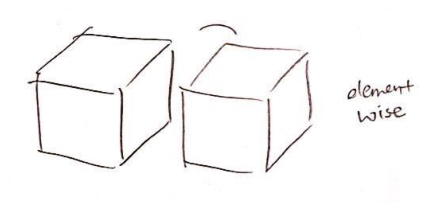
\includegraphics[height=8em]{resources/elementwise.png}
}{
  \begin{itemizec}
    \item $broadcastable(|x|, |y|)$
    \item $\mtt{.mean}$에 대해서는 텐서 타입이 floating이어야 함
  \end{itemizec}
}{
  \begin{itemizec}
    \item $broadcast(|x|, |y|)$
  \end{itemizec}
}{
  \begin{itemizec}
    \item 두 텐서의 elementwise 합/평균
  \end{itemizec}
}
\begin{align*}
  \forall \mtt{ft} \in \{\mtt{sum}, \mtt{mean}\},
  \bigspace
  \frac
  {
    \sigma \vdash \op{ft}{E, X} \Rar e, c
  }
  {
    \sigma \vdash \op{ft}{E, X, False} \Rar e, c
  }
\end{align*}%}}}

\subsection*{\texttt{torch.nn.Conv2d}}%{{{
\prepostc{torch.nn.Conv2d(in, out, kernel\_size, stride=1, padding=0,
dilation=1, groups=1)}{
  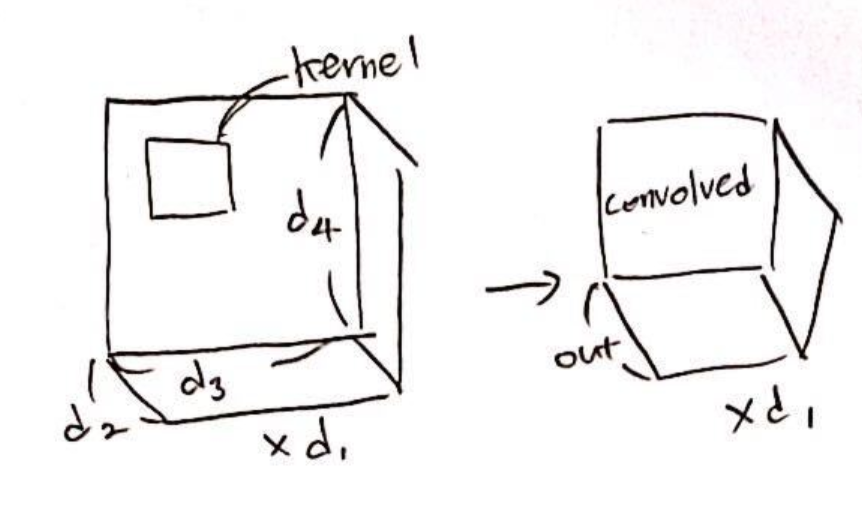
\includegraphics[height=12em]{resources/conv2d.png}
}{
  \begin{itemizec}
    \item $|x| = (d_1, d_2, d_3, d_4)$\bigspace ($rank = 4$)
    \item $d_2 = in$
    \item $kernel\_size[0] \leq d_3 + 2 \x padding[0]$
    \item $kernel\_size[1] \leq d_4 + 2 \x padding[1]$
    \item $groups | in$ and $groups | out$
  \end{itemizec}
}{
  \begin{itemizec}
    \item $(d_1, out, h, w)$ where.. refers to the proof tree.
  \end{itemizec}
}{
  \begin{itemizec}
    \item Convolution layer입니다. 선배님의 자료를 \ttt{pytorch}의 사용에 맞게
    풀어 쓴 것입니다.
  \end{itemizec}
}
\begin{align*}
  \frac
  {
    \begin{array}{l}
      \sigma \vdash E \Rar e, c \\
      k = \op{rank}{e} \\
      h = \left\lfloor \frac{e[3] + 2 \x padding \ind{0} - dilation \ind{0}
        \x (kernel\_size \ind{0} - 1) - 1}{stride \ind{0}} \right\rfloor + 1 \\
      w = \left\lfloor \frac{e[4] + 2 \x padding \ind{1} - dilation \ind{1}
        \x (kernel\_size \ind{1} - 1) - 1}{stride \ind{1}} \right\rfloor + 1 \\
      e' = (e[1], out, h, w) \\
      c_{dim} = \{ (k = 4) \land (e[2] = in) \} \\
      c_w = \{ (kernel\_size\ind{0} \leq e[3] + 2 \x padding \ind{0}) \} \\
      c_h = \{ (kernel\_size\ind{1} \leq e[4] + 2 \x padding \ind{1}) \} \\
      c_{group} = \{ (in \rem groups = 0) \land (out \rem groups = 0) \}
    \end{array}
  }
  {
    \sigma \vdash \module{Conv2d}{in, out, kernel\_size, stride=1, padding=0,
      dilation=1, groups=1}{E} \Rar e', c \cup c_{dim} \cup c_w \cup c_h \cup
      c_{group}
  } \\
  \\
  \text{$kernel\_size, stride, padding, dilation$는 가로-세로별 2-tuple로도 들어갈
  수 있음} \\
  \text{이 경우를 위해 $stride\ind{0}, stride\ind{1}$으로 표기함} \\
  \text{만일 $stride$가 튜플이 아닌 스칼라라면 $stride\ind{0}$ 또는 $\ind{1}$은
    $stride$ 값 자체를 의미}
\end{align*}%}}}

\subsection*{\texttt{torch.nn.MaxPool2d}}%{{{
\prepostc{torch.nn.MaxPool2d(kernel\_size, stride=kernel\_size,
padding=0, dilation=1)}{
  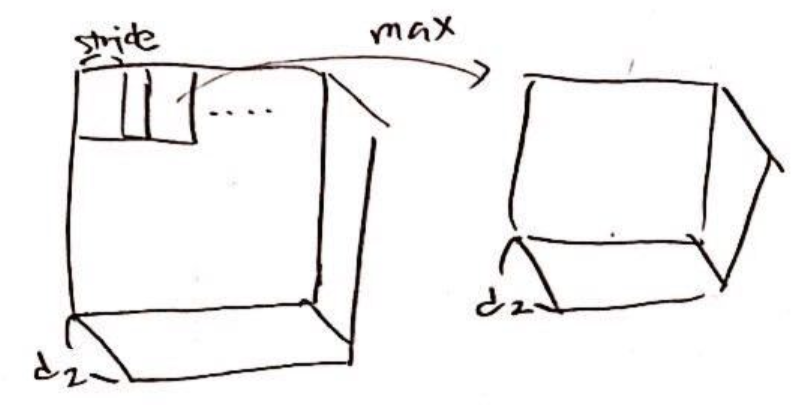
\includegraphics[height=10em]{resources/maxpool2d.png}
}{
  \begin{itemizec}
    \item $|x| = (d_1, d_2, d_3, d_4)\text{ or } (d_2, d_3, d_4)$
    \item $kernel\_size[0] \leq d_3 + 2 \x padding[0]$
    \item $kernel\_size[1] \leq d_4 + 2 \x padding[1]$
  \end{itemizec}
}{
  \begin{itemizec}
    \item $(d_1, d_2, h, w) \text{ or } (d_2, h, w)$ where.. proof tree.
  \end{itemizec}
}{
  \begin{itemizec}
    \item Convolution 다음 activation으로 자주 쓰이는 MaxPool 레이어 입니다.
  \end{itemizec}
}
\begin{align*}
  \frac
  {
    \begin{array}{l}
      \sigma \vdash E \Rar e, c \\
      k = \op{rank}{e} \\
      h_{orig} = e[k-1] \\
      w_{orig} = e[k] \\
      h = \left\lfloor \frac{h_{orig} + 2 \x padding \ind{0} - dilation \ind{0}
        \x (kernel\_size \ind{0} - 1) - 1}{stride \ind{0}} \right\rfloor + 1 \\
      w = \left\lfloor \frac{w_{orig} + 2 \x padding \ind{1} - dilation \ind{1}
        \x (kernel\_size \ind{1} - 1) - 1}{stride \ind{1}} \right\rfloor + 1 \\
      e' = e\indr{1}{k-2} \conc (h, w) \\
      c_{dim} = \{ (k = 3 \lor k = 4) \} \\
      c_w = \{ (kernel\_size\ind{0} \leq h_{orig} + 2 \x padding \ind{0}) \} \\
      c_h = \{ (kernel\_size\ind{1} \leq w_{orig} + 2 \x padding \ind{1}) \} 
    \end{array}
  }
  {
    \begin{array}{c}
      \sigma \vdash \module{MaxPool2d}{kernel\_size, stride=kernel\_size,
        padding=0, dilation=1}{E}
        \Rar e', c \cup c_{dim} \cup c_w \cup c_h 
    \end{array}
  } \\
  \\
  \text{$kernel\_size, stride, padding, dilation$는 가로-세로별 2-tuple로도 들어갈
  수 있음} \\
  \text{이 경우를 위해 $stride\ind{0}, stride\ind{1}$으로 표기함} \\
  \text{만일 $stride$가 튜플이 아닌 스칼라라면 $stride\ind{0}$ 또는 $\ind{1}$은
    $stride$ 값 자체를 의미}
\end{align*}

\prepost{torch.nn.MaxPool2d(kernel\_size, stride=..., dilation=1,
return\_indices=False, ceil\_mode=False)}{
  
\includegraphics[height=8em]{resources/maxpool2d_ri.png}
}{
  \begin{itemizec}
    \item $|x| = (d_1, d_2, d_3, d_4)\text{ or } (d_2, d_3, d_4)$
    \item $kernel\_size[0] \leq d_3 + 2 \x padding[0]$
    \item $kernel\_size[1] \leq d_4 + 2 \x padding[1]$
  \end{itemizec}
}{
  \begin{itemizec}
    \item $(d_1, d_2, h, w) \text{ or } (d_2, h, w)$ where.. proof tree.
    \item $return\_indices$가 $True$이면 인덱스 번호까지 튜플로 반환
    \item $ceil\_mode$가 $True$이면 $floor$대신 $ceil$로 shape 계산
  \end{itemizec}
}
\begin{align*}
  \frac
  {
    \begin{array}{l}
      \sigma \vdash E \Rar e, c \\
      k = \op{rank}{e} \\
      h_{orig} = e[k-1] \\
      w_{orig} = e[k] \\
      h = \left\lfloor \frac{h_{orig} + 2 \x padding \ind{0} - dilation \ind{0}
        \x (kernel\_size \ind{0} - 1) - 1}{stride \ind{0}} \right\rfloor + 1 \\
      w = \left\lfloor \frac{w_{orig} + 2 \x padding \ind{1} - dilation \ind{1}
        \x (kernel\_size \ind{1} - 1) - 1}{stride \ind{1}} \right\rfloor + 1 \\
      h_{ceil} = \left\lceil \frac{h_{orig} + 2 \x padding \ind{0} - dilation \ind{0}
        \x (kernel\_size \ind{0} - 1) - 1}{stride \ind{0}} \right\rceil + 1 \\
      w_{ceil} = \left\lceil \frac{w_{orig} + 2 \x padding \ind{1} - dilation \ind{1}
        \x (kernel\_size \ind{1} - 1) - 1}{stride \ind{1}} \right\rceil + 1 \\
      e' = \ifs{ceil\_mode}{e\indr{1}{k-2} \conc (h_{ceil},
      w_{ceil})}{e\indr{1}{k-2} \conc (h, w)} \\
      e_{out} = \ifs{return\_indices}{(e', e')}{e'}\\
      c_{dim} = \{ (k = 3 \lor k = 4) \} \\
      c_w = \{ (kernel\_size\ind{0} \leq e[3] + 2 \x padding \ind{0}) \} \\
      c_h = \{ (kernel\_size\ind{1} \leq e[4] + 2 \x padding \ind{1}) \} 
    \end{array}
  }
  {
    \begin{array}{rl}
      \sigma \vdash & \module{MaxPool2d}{kernel\_size, stride, padding,
        dilation, return\_indices, ceil\_mode}{E} \\
      & \Rar e', c \cup c_{dim} \cup c_w \cup c_h 
    \end{array}
  } \\
  \\
  \text{$return\_indices$가 $True$이면 (결과, 인덱스) 튜플 형태로 반환}\\
  \text{$ceil\_mode$가 $True$이면 $floor$대신 $ceil$함수로 계산}
\end{align*}%}}}

\end{document}
